\documentclass[12 pt]{article}
\usepackage[utf8]{inputenc}
\usepackage{matlab-prettifier}
\usepackage[portuguese]{babel}
\usepackage{indentfirst}
\usepackage{graphicx}
\usepackage{float}
\usepackage{subcaption}
\usepackage[font=small,labelfont=bf]{caption}
\definecolor{mygreen}{RGB}{28,172,0} % color values Red, Green, Blue
\definecolor{myyellow}{rgb}{1.0, 1.0, 0.8}
\usepackage{mathtools}
\usepackage{multirow}
\usepackage{comment}
\usepackage{xcolor}
\usepackage{colortbl}
\usepackage[normalem]{ulem}               % to striketrhourhg text
\usepackage{amsmath}
\usepackage{amsfonts}
\usepackage{hyperref}
\newcommand\redout{\bgroup\markoverwith
{\textcolor{red}{\rule[0.5ex]{2pt}{0.8pt}}}\ULon}
\renewcommand{\lstlistingname}{Código}% Listing -> Algorithm
\renewcommand{\lstlistlistingname}{Lista de \lstlistingname s}% List of Listings -> List of Algorithms

\usepackage[top=3cm,left=2cm,bottom=2cm, right=2cm]{geometry}
\usepackage{tikz}
\usetikzlibrary{decorations.pathreplacing}


% Configuração para destacar a sintaxe do Python
\lstset{ 
    language=Python,                     % A linguagem do código
    backgroundcolor=\color{myyellow}, % A cor do fundo 
    basicstyle=\ttfamily\footnotesize,   % O estilo do texto básico
    keywordstyle=\color{blue},           % Cor das palavras-chave
    stringstyle=\color{red},             % Cor das strings
    commentstyle=\color{mygreen},          % Cor dos comentários
    numbers=left,                        % Números das linhas à esquerda
    numberstyle=\tiny\color{gray},       % Estilo dos números das linhas
    stepnumber=1,                        % Número de linhas entre os números das linhas
    frame=single,                        % Moldura ao redor do código
    breaklines=true,                     % Quebra automática das linhas longas
    captionpos=t,                        % Posição da legenda
    showstringspaces=false               % Não mostra espaços em branco nas strings
    extendedchars=true,
    literate={º}{{${ }^{\underline{o}}$}}1 {á}{{\'a}}1 {à}{{\`a}}1 {ã}{{\~a}}1 {é}{{\'e}}1 {É}{{\'E}}1 {ê}{{\^e}}1 {ë}{{\"e}}1 {í}{{\'i}}1 {ç}{{\c{c}}}1 {Ç}{{\c{C}}}1 {õ}{{\~o}}1 {ó}{{\'o}}1 {ô}{{\^o}}1 {ú}{{\'u}}1 {â}{{\^a}}1 {~}{{$\sim$}}1
}


\title{%
\textbf{\huge Universidade Federal do Rio de Janeiro} \par
\textbf{\LARGE Instituto Alberto Luiz Coimbra de Pós-Graduação e Pesquisa de Engenharia} \par

\includegraphics[width=8cm]{COPPE UFRJ.png} \par
\textbf{Programa de Engenharia de Sistemas e Computação} \par
\large
CPS769 - Introdução à Inteligência Artificial e Aprendizagem Generativa \newline \par
\small
Prof. Dr. Edmundo de Souza e Silva (PESC/COPPE/UFRJ)\par 
Profa. Dra. Rosa M. Leão (PESC/COPPE/UFRJ)\par 
Participação Especial: Gaspare Bruno (Diretor Inovação, ANLIX) \par

\vspace{1\baselineskip}
\Large
\textbf{\textit{Lista de Exercícios 2
}}
}

\author{Luiz Henrique Souza Caldas\\email: lhscaldas@cos.ufrj.br}

\date{\today}

\begin{document}
\maketitle

\section*{Questão 1}

O objetivo deste trabalho é entender como construir um modelo preditivo simples (de Redes Neurais) usando uma ou mais camadas ocultas, e se familiarizar com os códigos em Python. Nesta tarefa, você deverá construir um modelo de rede neural simples para prever a nota de cada aluno em uma turma com base em duas features:

\begin{itemize}
    \item Fração de palestras assistidas
    \item Número de horas estudadas por semana (até o máximo de 8 horas em uma semana).
\end{itemize}

Sobre a Rede Neural e programa:

\begin{itemize}
    \item A sua rede neural deverá ter uma camada oculta com 3 neurônios. Portanto teremos 2 entradas (as 2 features), uma camada oculta e, na camada de saída, um neurônio.
    \item Os dados de entrada são fornecidos em uma planilha .ods (libreoffice), com os dados de 500 estudantes.
    \item Uma vez lido, o seu dataset deve ser aleatoriamente dividido de forma a que 80\% seja para treino do modelo e os restantes 20\% para teste.
    \item No seu programa:
    \begin{itemize}
        \item Use um Scaler padrão do sklearn para dimensionar os dados de treinamento. Explique o motivo de escalonar os dados de entrada.
        
        \textbf{Explicação:} \par

        Escalonar os dados de entrada normaliza suas distribuições, levando a média para zero e o desvio padrão para o valor unitário, permitindo uma convergência mais rápida e estável do modelo de machine learning, pois o modelo não precisa lidar com features de ordem de grandeza diferentes.

        \item Para a camada oculta, use a função de ativação ReLU (Rectified Linear Unit).
        \item A camada de saída usa a ativação linear padrão (explique o que é).
        
        \textbf{Explicação:} \par

        A ativação linear padrão retorna a entrada sem modificações ($f(x)=x$), usada em problemas de regressão para prever valores contínuos.

        \item Use o algoritmo de otimização Adam (Adaptive Moment Estimation). Explique bem resumidamente as vantagens em relação ao Stochastic Gradient Descent padrão.
        
        \textbf{Explicação:} \par

        Adam ajusta a taxa de aprendizagem para cada parâmetro individualmente e utiliza momentos dos gradientes, permitindo convergência mais rápida e estável.

        \item Use mean square error para a função de perda. Explique bem resumidamente o objetivo da função de perda.
          
        \textbf{Explicação:} \par

        A função de perda mede a diferença entre as previsões do modelo e os valores reais. Durante o aprendizado, o ajuste dos pesos é feito de forma a minimizar o valor da função de perda, melhorando a acurácia do modelo.

    \end{itemize}
\end{itemize}

Responda:

\begin{enumerate}
    \item Como o modelo de rede neural está estruturado? Explique a arquitetura.
    
    \textbf{Resposta:} \par

    O modelo possui duas entradas (as duas features), uma camada oculta com 3 neurônios usando a função de ativação ReLU, e uma camada de saída com um neurônio e ativação linear.

    \item Explique o papel da função de ativação usada na camada oculta.
   
    \textbf{Resposta:} \par

    A função ReLU (Rectified Linear Unit) ajuda a introduzir não-linearidade ao modelo, permitindo que ele aprenda relações complexas entre as entradas e as saídas.

    \item Treine o modelo com o conjunto de dados fornecido. Qual o erro quadrático médio nos dados de teste?
       
    \textbf{Resposta:} \par

    O modelo foi treinado por 600 épocas e no conjunto de teste o menor erro médio quadrático obtido foi de \textbf{$307.94$}.

    \item Trace o erro quadrático médio em função das “épocas” (dos passos para a convergência). Descreva a tendência que você observa.
       
    \textbf{Resposta:} \par

    \begin{figure}[H]
        \caption{Eveloução do erro de treinamento ao longo das épocas.}
           \centering
           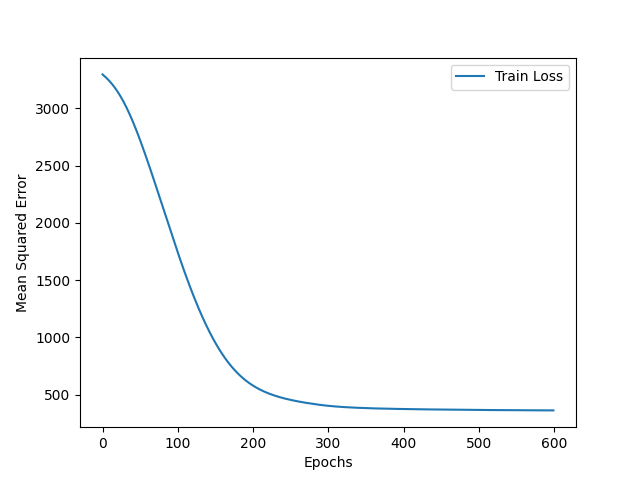
\includegraphics[height=8cm]{fig/item_4.png}
    \end{figure}

    Pelo gráfico acima, é posssível observar que o erro médio quadrático tende a cair com o aumento das épocas até que esta queda deixa de ser relevante, o que ocorre por volta de 400 épocas.

    \item Mostre os pesos e bias de cada camada após o treinamento, isto é, mostre os parâmetros aprendidos do modelo.
       
    \textbf{Resposta:} \par

    \begin{table}[H]
        \centering
        \caption{Pesos e Bias das Camadas}
        \begin{tabular}{|c|c|l|}
            \hline
            \textbf{Camada} & \textbf{Tipo} & \textbf{Valores} \\
            \hline
            \multirow{2}{*}{1} & Pesos & 2.3686342 | 2.3783615 | 0.71419466 \\
                               &       & 2.0336158 | -2.3631034 | 1.5801256 \\
            \hline
            1 & Bias   & 3.7342753 | 4.462739 | 4.0898366 \\
            \hline
            2 & Pesos & 4.112546 | 3.063474 | 4.479588 \\
            \hline
            2 & Bias   & 2.6367683 \\
            \hline
        \end{tabular}
    \end{table}

    \item Use o modelo treinado para prever as notas a partir dos dados de novos alunos (com um segundo dataset fornecido sem as notas). Mostre as previsões feitas pelo modelo e explique os resultados.
       
    \textbf{Resposta:} \par

    \begin{table}[H]
        \centering
        \caption{Resultados da previsão a partir dos dados de novos alunos.}
        \begin{tabular}{|c|c|c|}
            \hline
            \textbf{Presença} & \textbf{HorasEstudo} & \textbf{Nota} \\
            \hline
            0.3745401188 & 2.974337759 & 32.95745 \\
            \hline
            0.9507143064 & 5.628494665 & 82.800064 \\
            \hline
            0.7319939418 & 3.183951849 & 57.951267 \\
            \hline
            0.5986584842 & 2.175392597 & 44.790115 \\
            \hline
            0.1560186404 & 7.931297538 & 44.161804 \\
            \hline
            0.1559945203 & 4.548447399 & 24.69879 \\
            \hline
            0.05808361217 & 5.135056409 & 20.509508 \\
            \hline
            0.8661761458 & 2.150503628 & 62.7456 \\
            \hline
            0.6011150117 & 3.911234551 & 52.116886 \\
            \hline
            0.7080725778 & 5.221845179 & 64.74353 \\
            \hline
            0.0205844943 & 2.698012845 & 17.904613 \\
            \hline
            0.9699098522 & 5.751396037 & 84.60283 \\
            \hline
            0.8324426408 & 3.79872262 & 67.26796 \\
            \hline
            0.2123391107 & 4.4166125 & 27.958336 \\
            \hline
            0.1818249672 & 3.796586776 & 23.457981 \\
            \hline
            0.1834045099 & 8.704556369 & 51.34989 \\
            \hline
            0.304242243  & 4.973005551 & 36.457355 \\
            \hline
            0.5247564316 & 2.884578142 & 42.72716 \\
            \hline
            0.4319450186 & 6.645089824 & 51.97556 \\
            \hline
            0.2912291402 & 2.5583127   & 27.386648 \\
            \hline
        \end{tabular}
    \end{table}

    \item Modifique o programa para adicionar mais camadas e/ou maior número de neurônios ocultos. Como suas modificações afetam o desempenho do modelo?
    
       
    \textbf{Resposta:} \par

    Foram testados dois novos modelos, um com 3 camadas ocultas com 3 neurônios cada e outro com uma camada oculta com 9 neurônios. 

    Enquanto o modelo original (uma camada oculta com 3 neurônios) obteve um erro médio quadrático de $307.94$, o modelo de 3 camadas de 3 neurônios obteve um erro de $315.00$ e o modelo com uma camada de 9 neurônios obteve um erro de $309.56$.

    Foi testado então um novo modelo com uma camada oculta de 100 neurônios (valor padrão do tensor flow). O erro médio quadrático obtido foi de $312.28$.

    Nenhuma das 3 novas arquiterturas testadas superou o desempenho da arquitetura original, com uma camada oculta de 3 neurônios. 

    \item Quais seriam algumas melhorias potenciais ou recursos adicionais que poderiam ser adicionados ao modelo para melhorar sua precisão preditiva?
    
       
    \textbf{Resposta:} \par

    Para melhorar a precisão preditiva, poderia-se adicionar regularização (como Dropout), usar técnicas de aumento de dados, ou experimentar diferentes arquiteturas de rede.

    \item Faria sentido usar a função de ativação sigmoid no modelo? Explique em poucas palavras.
       
    \textbf{Resposta:} \par

    A função sigmoid é mais adequada para tarefas de classificação binária. Para problemas de regressão, como o apresentado, a ativação linear na saída é mais apropriada.

\end{enumerate}

\section*{Código}

O código abaixo encontra-se no repositório \href{https://github.com/lhscaldas/cps769-ai-gen}{https://github.com/lhscaldas/cps769-ai-gen}, bem como o arquivo LaTex com o relatório.


\lstinputlisting[language=Python,caption=código fornecido completo com algumas modificações]{Lista_2.py}

\end{document}